After building up intuition on the biological features of a Drosophila embryo and a model capable of (somewhat crudely) mimicking it, we can now begin probing our model for interesting phenomena. We know that cells in nature act by relatively simple, local rules. Having added a minimal number of these in our simulation, we would like to see whether it can model gastrulation reminiscent of what is seen in vivo. Focusing not just the final structures, but also the individual events leading up to it. \\

Once we have assessed the phenomenological validity of our model, we will look onward for intriguing phenomena to study. Given our full embryo model from we will be looking into the interplay between the different active domains and events.\\


On the structure: In the following sections we will go through the similarities between simulation and reality, starting from simple visual comparisons, ending in detailed quantifications. We will do these for the different events (\vf{A1}, \gb{A2} and \pmg{A3}) and embryo domains. Afterwards, we will be looking at removing different active parts of the simulated embryo, comparing the results to known real-life mutants. This will finally lead us to a purely in-silico analysis of the interaction between spatially distinct [domains] of the embryo.\\ 

\renewcommand{\contentsname}{Results Section Table of Contents}
 \setcounter{tocdepth}{3}
\localtableofcontents
\renewcommand{\contentsname}{Table of Contents}
 \setcounter{tocdepth}{1} 


\newpage

\section{Qualitative Agreement}
While the Drosophila embryo has been studied for decades, it is only relatively recently that microscopy and computer science has gotten to a point where quantitative analyses of the more than 5000 cells have become feasible. Therefore, like in most of the fields history, we will start with visually examining the morphology of the embryo. 

For all figures in this paper, If nothing else is noted, the run is [define run]. In vivo, the time of invagination of the posterior midgut (\pmg{A3} in the overview) is about 12 minutes after start, the timing of the simulation is defined to align with this event, allowing for direct comparisons in "minutes" across simulated and experimental timelines.\\


We will start out this section with an overview which we compare to imaged embryos to ensure that there is general phenomenological agreement. We will then go through the individual main morphological events (\vf{A1}, \gb{A2} and \pmg{A3} from Figure \ref{fig:big-timeline}) and qualitatively assess the resemblance between the simulated events and real embryos, hopefully providing some preliminary insight into the [simulated] mechanics. Finally, we will make some additional visual annotations to aid in estimating the nature of the tissue movements, which will help facilitating a more intuitive understanding of these developmental changes.

On the following page, we [compare] our best in silico model and corresponding frames from a video by [Stas' group]: \todo{more specific about video, and explain visuals succinctly}
\newpage

\begin{figure}[H]
    \centering
    \vspace*{-1cm}\hspace*{-1cm}\makebox[\textwidth]{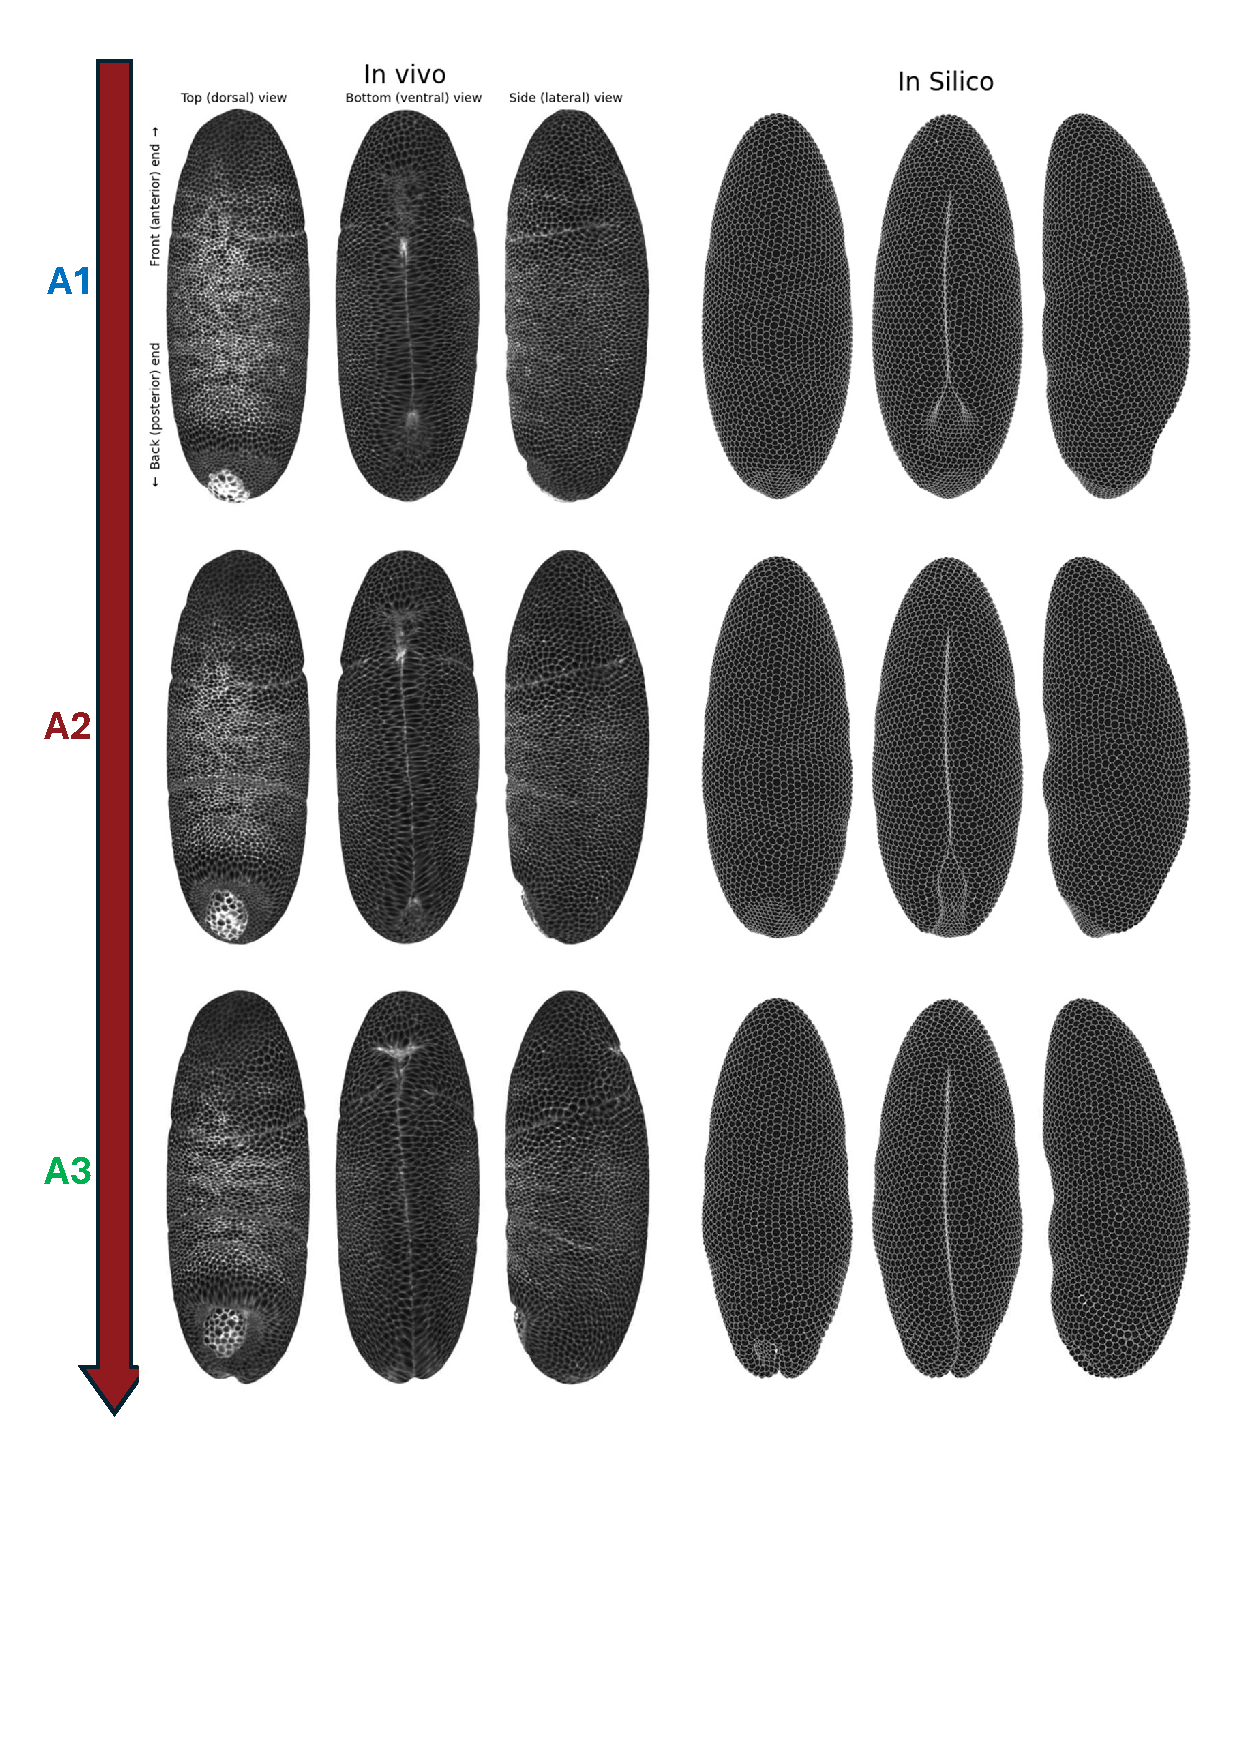
\includegraphics[width=0.85\paperwidth]{chapters/Results/figures/compare_to_vid_timeline_v2.pdf}}
    \caption{Caption on next page}
    \label{fig:big-visual-comparison}
\end{figure}
\newpage
\addtocounter{figure}{-1}
\begin{figure} [t!]
  \caption{(Previous page.) \\A full page visualization of three time steps of the simulation and corresponding point from in vivo imaging. 
  Each row consists of a single time-step and corresponds roughly to the three previously highlighted primary events (\vf{A1}, \gb{A2} and \pmg{A3}). Within each row, the embryo is show from the top (dorsally), bottom (ventrally), and side (laterally), with the back end (posterior) pointing downwards.
  A cursory comparison reveals a general alignment in the overall morphologies.\\
  \textbf{Left:} In vivo imaging with cell walls highlighted by use of a membrane marker (Source: \citeAY{stern2022deconstructing}).\\ \textbf{Right:} In silico visualization. For ease of comparison the colors have been made to match the data.}
\end{figure}


It is easy to hide behind numbers and advanced analytical methods, so for completeness sake we have started by presenting a visually unaltered full-scale comparison. Our analyses will soon be more sophisticated, but from a naive inspection, the general dynamics, timing and shape seems to generally have been recapitulated. Given the relatively simple model and few specific alterations, this is already notable! we can see that ... \\ 


To completely understand the agreements between data and simulation we will need to scrutinize the individual pieces using some visual aids. Using the main events (\vf{A1}, \gb{A2}, \pmg{A3}) as starting points, we will go to a higher level of resolution, focusing on individual parts of the embryo, validating the simulation and comparing them to in-vivo imaging when available.


\subsection{(\vf{A1}) Ventral Furrow }
The the first sign of movement on the embryo is on the belly where a distinct cleft begins forming. \\
This is called the \vf{ventral furrow} and is an important part of creating the gastrointestinal tract.

From Figure \ref{fig:big-visual-comparison} we have from an external perspective seen the characteristic cleft form on the bottom side, mirroring the initial stages of invagination. The furrow closes off in just over three minutes.\cite{holly2015rapid}
As the furrow closes, the internalized cells form a tube with a recognizable light bulb-shape in the cross section. \\

Below, in Figure \ref{fig:VFComparison}, a comparison between a cross section of our simulation and in vivo imaging can be seen.

\begin{figure}[H]
    \centering
    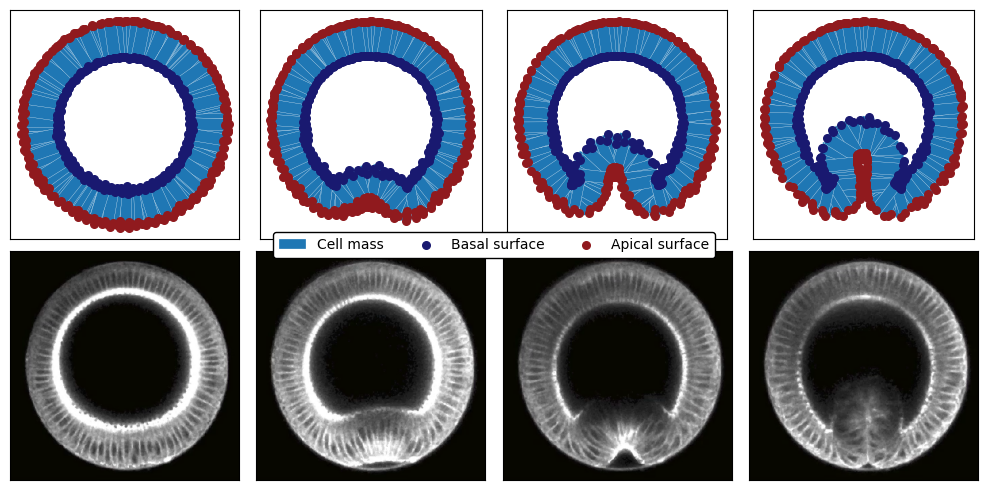
\includegraphics[width=1\linewidth]{chapters/Results/figures/VF_comparison.png}
    \caption{A comparison of cross sections showing the dynamic morphology of the ventral furrow formation (\vf{A1}) in simulation (\textbf{upper row} and frames from video of live growth (\textbf{lower row}). For ease of comparison, each cell in the simulation is displayed as a rectangle with the longer side aligning with its simulated apical-basal-axis. The blue and red dots are approximations of the inner and outer cell walls, also calculated using their apical-basal polarities. The cutting plane used in simulation can be seen in Figure \ref{fig:cutplane}. The video is multi-photon microscopy of cell walls (Source: \citeAY{conte2012biomechanical})}
    \label{fig:VFComparison}
\end{figure}
%  $\textbf{r} + a\textbf{p}$ and $\textbf{r}-a\textbf{p}$ respectively (for position $\textbf{r}$ and AB-vector $\textbf{p}$ and some scale constant \textit{a}). 
\begin{figure}
    \centering
    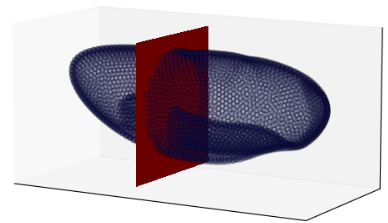
\includegraphics[width=0.8\linewidth]{chapters/Results/figures/planecut2.png}
    \caption{The cutting plane used for visualization in Figure \ref{fig:VFComparison} visualized.}
    \label{fig:cutplane}
\end{figure}
Overall, both the motion observed during development and the final shape of the structure appear to be well aligned with the in-vivo observations.\\

In simulation, we can visually observe the same dynamic process of ventral furrow formation, with remarkable parallels to what occurs in the embryo (\vf{A1}). In Figure \ref{fig:VFComparison} we can now see, that as the simulation progresses, the closure of the furrow and internalization of cells produce the familiar tube-like structure, with the cross-section displaying the previously mentioned light bulb-shaped profile. While our simulation progresses about 50\% too fast (the closing takes 2 minutes instead of 3), we notice that the relative/interal timing is accurately captured. Adding to this, the directions of movement and rotation of apical- and basal sides of each cell closely match what is observed in real embryos, further validating its accuracy. \\

In our simulation, the invaginating tissue extends slightly more towards the center. This is especially noticeable closer to the head (anterior tip) (see Section \ref{App:VF} in the Appendix).\todo{Add to appendix!} This problem also plagues the state of the art \citeAY{allena2010simulation} who did a full vertex-based simulation focusing on the ventral furrow. This common difficulty might stem from the fact that after closing, the ventral furrow starts 'pinching off' disconnecting the internalized cells which includes some dynamics not present in the simulations.\cite{supatto2008quantitative}\\
In general, we find the first key morphogenetic event (\vf{A1}) -- the formation of the ventral furrow --  to have been adequately recreated.

\subsection{(\gb{A2}) Germ-band}
The most numerous cell group we are interested in is the \gb{germ-band} which fill most of the lateral sides. As mentioned in Section \ref{sec:ConvergentExtension}, it is generally agreed that the germ-band is one of the main drivers of horizontal motion, although it remains disputed how.

In Figure \ref{fig:germbandCompare} a text-book diagram of the motion of the germ-band can be compared with the shape of the germ-band in the first and last frame of our simulation. 
\begin{figure}[H]
    \centering
    \begin{subfigure}[b]{0.3\textwidth}
        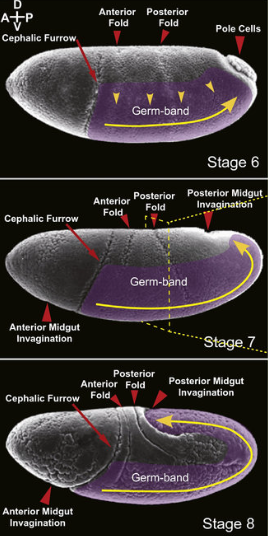
\includegraphics[width=\textwidth]{chapters/Results/figures/compareGB.png}
    \caption{}
    \end{subfigure}
     % \hfill
    \begin{subfigure}[b]{0.61\textwidth}
    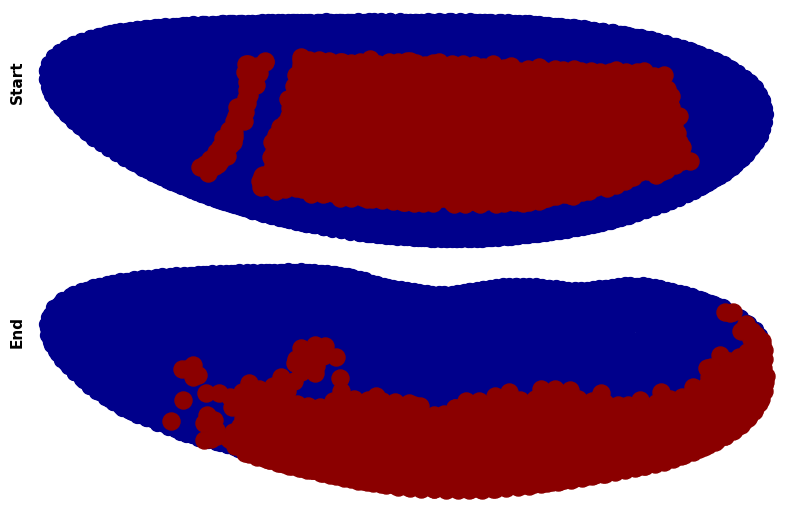
\includegraphics[width=\textwidth]{chapters/Results/figures/gb_firstframe_lastframe.png}
    \caption{}
    \end{subfigure}
    \caption{\\
    \textbf{(a)} A diagram of the germ-band (purple shaded area) and its motion when extending (\gb{A2}) (Source: \citeAY{kong2017forces})\\
    \textbf{(b)} Simulation with colored in germ-band at $t = 0 \text{ min}$ and $t \approx 15 \text{ min}$\\Note: The blue line separating the germ-band in the initial frame is a quirk of the gene-expression-cutoff as described in Section \ref{App:morphogens}.}
    \label{fig:germbandCompare}
\end{figure}



To reiterate, during gastrulation, the motion of the germ-band is as follows:\\Firstly, the tissue moves downward towards the invaginating ventral furrow (\vf{A1}), then extends horizontally, before ultimately curving upwards as it encounters the back (posterior) tip of the embryo.\\

In general, we see great agreement between simulation and data in the final shape and placement of the germ-band. This says nothing explicit about the timing and interaction of these activities present, but it hints at the fact that the movement towards the belly, back, and top side can also found in our model. To get a better understanding of the agreement, we will need to look at the active aspect of the germ-band extension.\\

Later we will have quantitative measures allowing for studying the temporal aspect, but for now, we can focus on a neat observation: The cells in the germ-band that start further towards the back will migrate much further horizontally than the cells closer to the head, with cells next to the \cephalic{cephalic furrow} only moving downwards (ventrally). This is a result of the extension being the sum of many small contributions adding to the global motion. 

For a representation of the motion of individual cells in the germ-band, a random selection can be seen in Figure \ref{fig:GBMovements} below:
\begin{figure}[H]
    \centering
    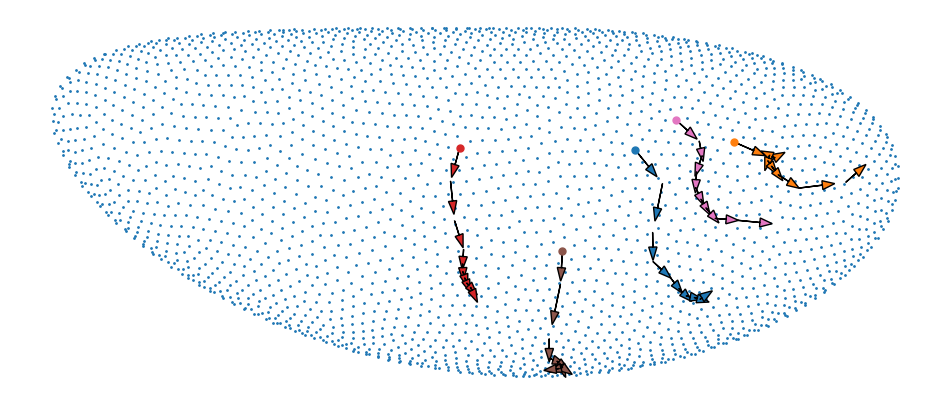
\includegraphics[width=1\linewidth]{chapters/Results/figures/movements.png}
    \caption{A number of cells from the germ-band with their migration over time visualized. The arrows correspond to movement in equally spaced time intervals during the germ-band extention (\gb{A2}).
    It can be seen that -- like in real embryos -- cells that are formed closer to the posterior tip migrate more in the horizontal than vertical direction.}
    \label{fig:GBMovements}
\end{figure}

It can be seen that we have captured the uneven cell migration, where cells that starts further along the horizontal axis along also moves more horizontally. 

For completeness sake, we have also made a stream-plot where, the flow field which is a way to visualize the individual motion of all cells at once. This can be seen in Figure \ref{fig:streamplot}:


\begin{figure}[H]
    \centering
    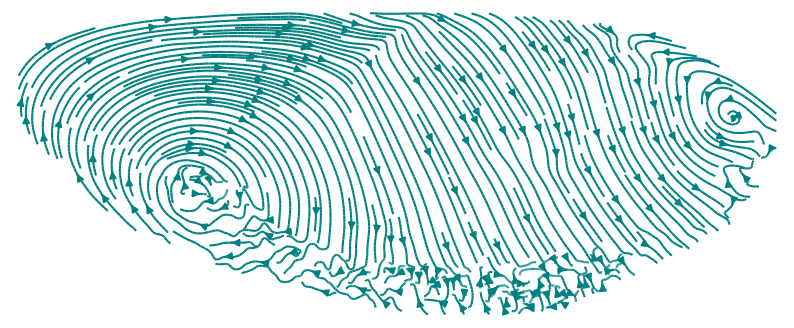
\includegraphics[width=1\linewidth]{chapters/Results/figures/streamplot2.png}
    \caption{\todo{make good?}}
    \label{fig:streamplot}
\end{figure}

Without any basis of comparison this flow-field is not [smth], but it looks cool so we kept it in.
We hope, that by capturing some of the aspects of the single-cell movements we have also caught some of the deeper, global dynamics of the tissue.\todo{finish or cut}\\

To summarize: We have a great visual agreement in the change of tissue-scale morphology of the germ band. The migration downwards towards the belly (ventral side) due to the furrow formation, the germ-band actuating horizontal motion, and finally the 'rise' at the back (posterior tip) due to the boundary condition, all seems to have been captured by the model. In the single-cell case we also see a general correspondence between simulation and reality, preliminarily supporting that the tissue behaves as expected.\\  


An examination of the dynamical timeline will have to wait till later sections, but in general, we find that our simulation has comparable morphological changes of the second main event, the germ-band extension (\gb{A2}).


\subsection{(\pmg{A3}) The Posterior Midgut Invagination }
Now, our final point of focus is also the hardest to visualize neatly. Looking at electron microscopy as below in Figure \ref{fig:PMG-IRL}, we can get a rough idea of the motion:
The back tip moves slightly upwards. Once it reaches a certain point, the tip folds in on itself as the ventral furrow reaches it, connecting the tube with the invaginating cavity.\cite{campos2013embryonic}

\begin{figure}[H]
    \centering
    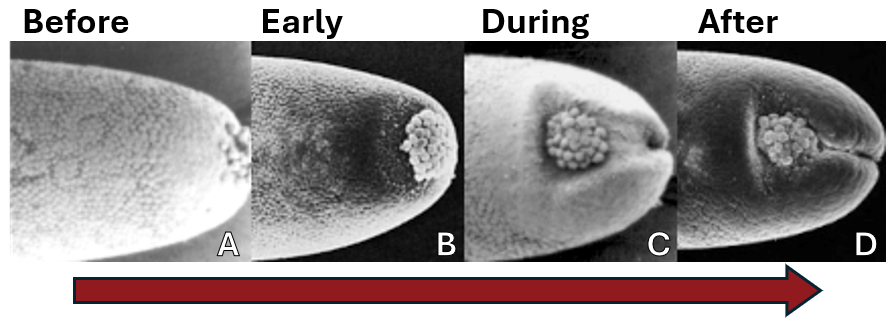
\includegraphics[width=1.\linewidth]{chapters/Results/figures/4stepPMG_annotated.png}
    \caption{An overview of the \textit{posterior midgut invagination} (\pmg{A3}) as viewed from the top (dorsal) side. \\The pole cells -- which are clearly visible at the posterior tip (\textbf{A}) -- are moved to the top and towards the front of the embryo (\textbf{B}). As the tissue beneath them apically constrict, the newly formed indent merge with the \vf{ventral furrow} as this reaches the posterior tip (\textbf{C}). Finally the pole cells are internalized as the furrow closes off (\textbf{D}).The time points are not linearly spaced.\\
    (Sources: \textbf{A \&} \textbf{C}: \citeAY{sweeton1991gastrulation}, \textbf{B \&} \textbf{D}: \citeAY{gibert1994genetics}}
    \label{fig:PMG-IRL}
\end{figure}
Zooming in on the very back of our simulated embryo, we can see much of the same dynamics represented:
\begin{figure}[H]
    \centering
    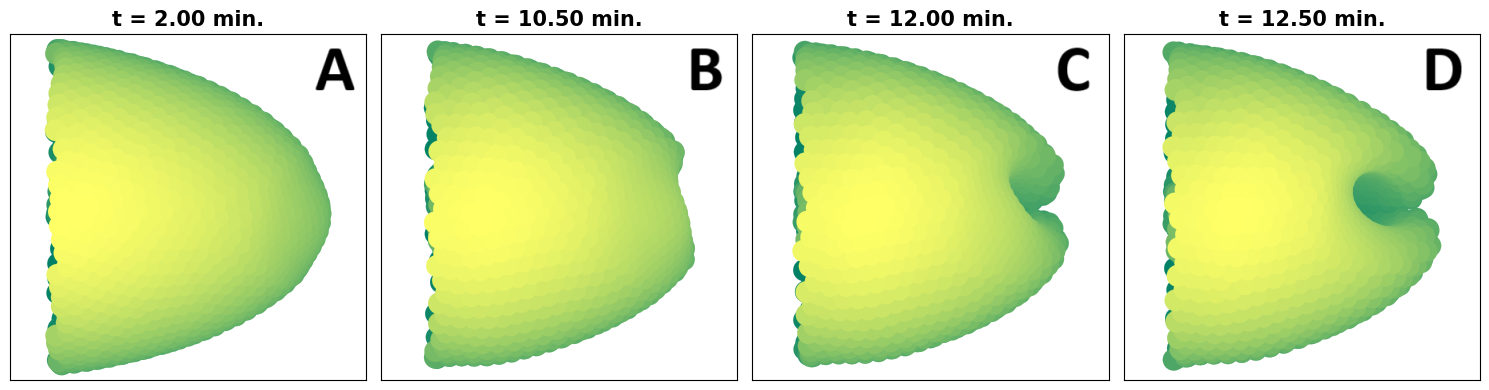
\includegraphics[width=1.\linewidth]{chapters/Results/figures/VisualPMG.png}
    \caption{A zoom-in on the the top side of the posterior tip of the embryo. To to be compared with Figure \ref{fig:PMG-IRL}. \\The PMG-event (\pmg{A3}) goes as follows: The cells in the tip starts tightening (\textbf{A}), the tip then is pushed upwards (\textbf{B}), it then invaginates meeting the ventral furrow comes from below (\textbf{C}) before being moved further up (\textbf{D}).}
    \label{fig:visual-pmg-external}
\end{figure}

The formation of the posterior midgut (\pmg{A3}) is an intensely studied phenomenon in Drosophila gastrulation, but has, to the best of our knowledge, not previously been simulated.

Visually grasping what happens in vivo can be tricky, as there is a distinct lack of good imaging of this phenomenon. This is caused by two things: The action happens very quickly (the fold buckles as a release of pressure) and much of the interesting cellular dynamics happens inside, or on the border of an invagination. This point will return shortly, but visually we seem to be agreeing with the external imaging for the most part. In general we capture the motion upwards followed by both a folding and a fusion. Unfortunately, in our simulation the upwards momentum is slowed to a halt -- in vivo, the posterior is moved much further after invagination. In dialogue with Nobel laureate Erik Wieschaus, we have found that the isotropy of our cell size might be to blame, as phenotypes with less cell-deformation experiences the same trouble.\todo{Keep? Remove?} This might be caused by the top (dorsal) part of the embryo not "moving out of the way" or the bottom (ventral) part not having the correct amount of pressu/force.\todo{Important - finish}\\

Our frustration with a lack of good reference images extends to the fact, that once invaginated, cells are impossible capture by ordinary microscopy and hard to automatically [define]. The only usable visualization of internalized cells, is of a meticulously \textit{hand-tracked} vertical band around the posterior tip. The approximate extend of this band can be seen here:
\begin{figure}[H]
    \centering
    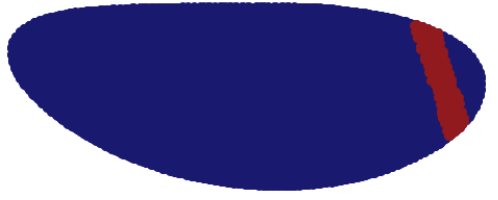
\includegraphics[width=0.5\linewidth]{chapters//Results//figures/daniel_band_pos.png}
    \caption{The approximate band as used in the following section for analyzing the deformations around the posterior midut.}
\end{figure}

As looking 'inside' our virtual embryo is trivial compared to real life, we have extracted the band of cells, trying to recreating the framing of the data. In Figure \ref{fig:daniel-cells} the collected data can be seen and in Figure \ref{fig:comparetodaniel} the geometrically[?] corresponding cells can be seen in simulation. 
\newpage
\begin{figure}[H]
    \centering
    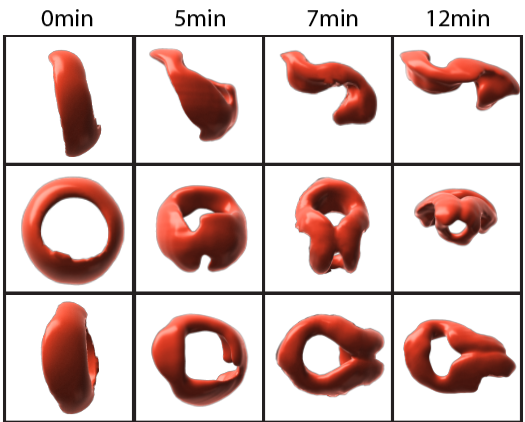
\includegraphics[width=0.7 \linewidth]{chapters/Results/figures/DanielCut.png}
    \caption{A 3D mesh of cells from in vivo imaging. Each row is a constant angle. (Source: Daniel Alber. Not yet published. Reproduced with permission)}
    \label{fig:daniel-cells}
\end{figure}
\begin{figure}[H]
    \centering
    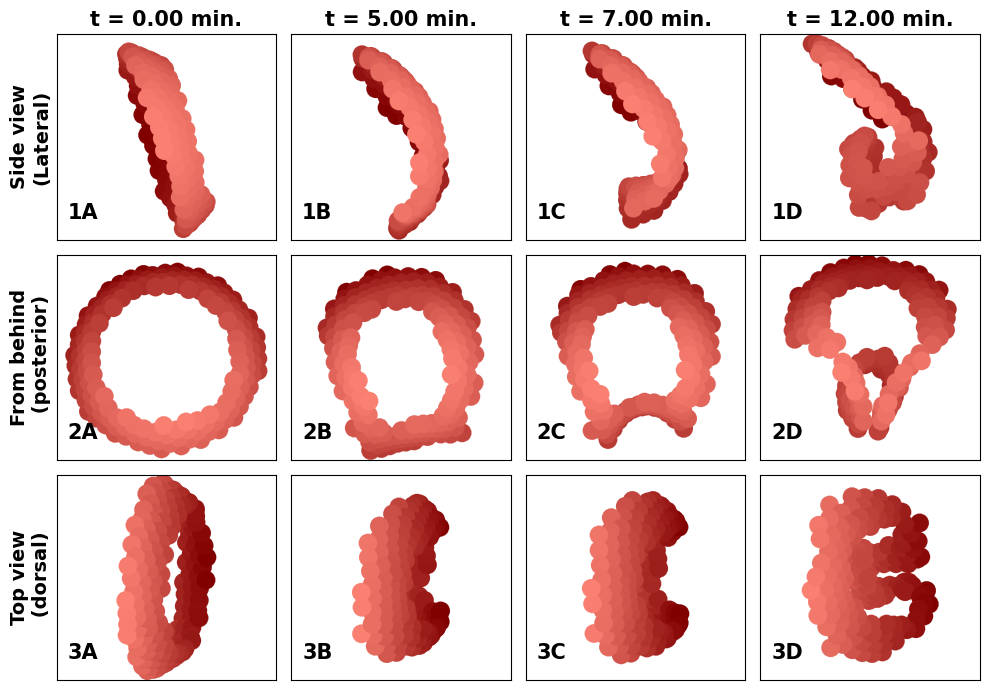
\includegraphics[width=0.8\linewidth]{chapters/Results/figures/CompareToDaniel.png}
    \caption{\todo{make cool 3D cells so it looks more like Figure \ref{fig:daniel-cells}?}}
    \label{fig:comparetodaniel}
\end{figure}

The combined invagination of the PMG and the ventral furrow (\pmg{A3}), is now easily visible in \textbf{2C-}\textbf{2D}. For the first 5-6 minutes of the timeline, simulation and reality are relatively well aligned. We see a push from the extending germ-band moving the cells towards the posterior tip. The trouble begins in \textbf{1C} and \textbf{1D} where the orientation of the cell-band should be almost horizontal. As Figure \ref{fig:comparetodaniel} shows, our model has not moved the cells far enough towards the top. In spite of this, as the posterior closes off, a YY right morphology emerge. It should also be noted that the closing happens at a reasonably YYY timing. In general a we have a respectable qualitative agreement, albeit the trouble the lack of upwards (dorsal) motion is visually evident.\\



Our model clearly has some fundamental flaw or inconsistency, but barring the lack of movement towards the back, we got quite close in both timing and shape. With a few exceptions, our model provides a phenomenologically faithful recreation of this vital morphogenetic event. As the posterior invagination (\pmg{A3}) requires both successful modeling of (\vf{A1}) and (\gb{A2}), we are, to the best of our knowledge, the first group to attempt an in silico [experiment]. So while our simulation is not perfect, the fact that this is a world-first attempt at something this well-studied is a  noteworthy [achievement(?)].\\

\todo{reread these last two paragraphs. I feel like I am rambling}
 

\subsection{General morphology}
In the literature, a way of visualizing changes in both local and global structure, consist of drawing virtual lines on an embryo at the onset of gastrulation. How these lines translate and skew over time is very descriptive for the general changes in form. An example in both data and simulation can be seen in Figure \ref{fig:band-movements-stas}.

\begin{figure}[H]
    \centering
    \makebox[\textwidth][c]{\hspace*{-1cm}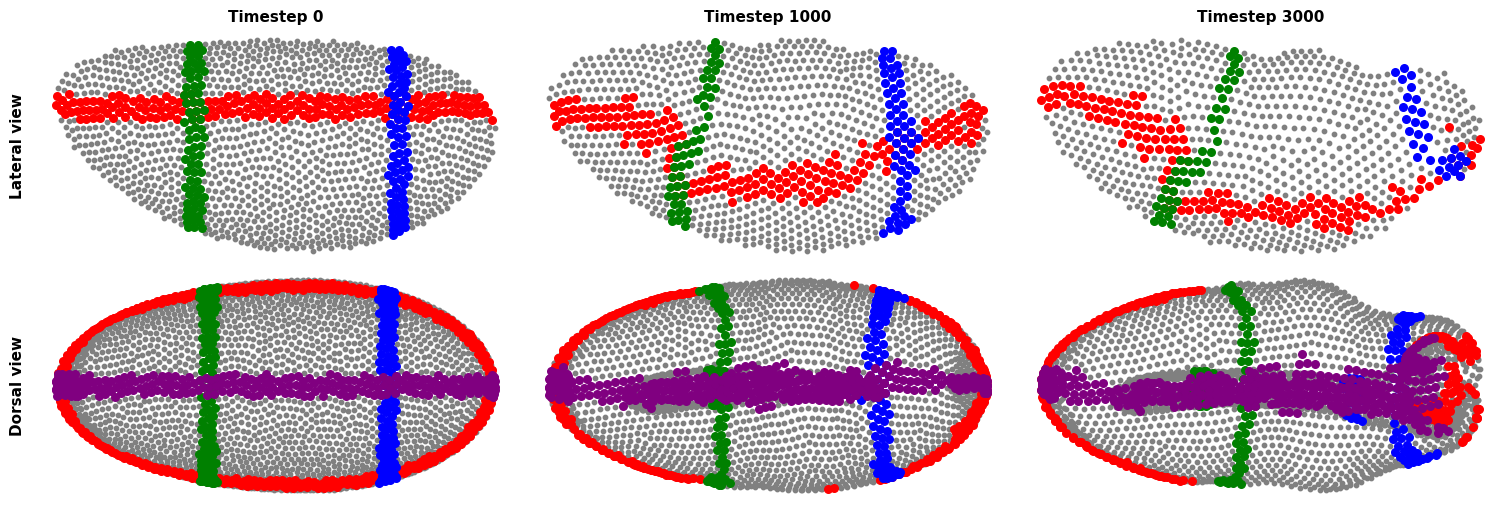
\includegraphics[width=1.\linewidth]{chapters/Results/figures/band_movements.png}}
    % \caption{My simulation. Compare to figure \ref{fig:band-movements-stas}}
    % \label{fig:band-movements}
\end{figure}
\begin{figure}[H]
    \centering
    \makebox[\textwidth][c]{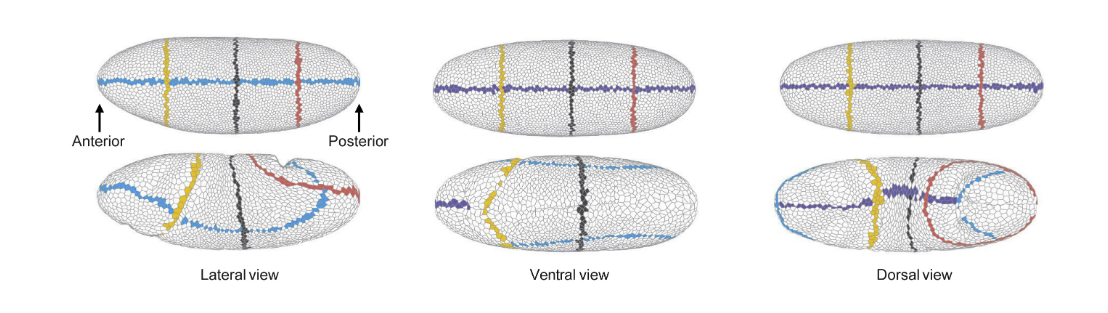
\includegraphics[width=1.\linewidth]{chapters/Results/figures/compareStasGBShape.png}}
    \caption{Positions of specific colored-in bands at two differnt time points.\\ 
    As can be seen, the general movements align quite well, albeit with some discrepancies around the posterior tip.
    \\ \textbf{Top row:} Simulation.\\ \textbf{Bottom row:}  Segmented images (Source: \citeAY{stern2022deconstructing}). \\\todo{write more!}}
    \label{fig:band-movements-stas}
\end{figure}

This juxtaposition allows for some interesting observations:\\
As is evident, there is a general agreement between both local and large-scale changes in embryonic form. \\

Going through the lines, color by color we might be able to surmise [smth] about the differences in dynamics between our model and [in vivo]:\todo{finish}

\begin{description}
   \item[\lightblue{Blue}] The biggest problem is also very evident plaguing our simulation is evident. The pressure from the bottom (ventral) side of the model cannot push the posterior tip. The blue line acts as a stand-in for the germ-band. Much of the analysis from its section applies with two exceptions:
   \begin{itemize}
       \item In simulation, close to the (deliberate) lack cephalic furrow (the \lightyellow{yellow} line), the blue line breaks up. \todo{write something about lack of pressure relief}   
       \item The second image is later than what we previously compard the germ-band to. Here the lack of upwards motion is (much like all the woke left) pronounced.\todo{make professional}
   \end{itemize}
   \item[\lightred{Red}] The same effect can also be seen in the red line, where it almost, but not [totally] reach the rightmost (posterior) tip. It can also be seen, that after invagination and the lines close to the end (red and blue) becomes muddled.
   \item[\lightyellow{Yellow}] A helpful line for understanding the motion around the area of the cephalic furrow. The top part moves towards the bacj and the bottom towards the front. Not too much bending. We have great agreement! 
   \item[\lightpurple{Purple}] The mid-line seems as stable as in vivo. The "bunching up" of the \lightpurple{purple} in the posterior-end is most likely an artifact from the fact, that -- unlike in real life -- the cells are not being hidden below other tissue in the posterior invagination.
\end{description}


fault lines er godt ord

We will discuss this later, but a possible root of the problem is also a lack of flexibility in the top (dorsal) tissue. This most likely stems from a lack of [Dorsal Transverse Folds]. \todo{finish though, mention pre-print?}

Other observations:
The point cloud of our 'cells' become spread out in a way that mirrors the individual cells quite radical surface area increase after room has been made by the various invaginated tissue. 


Quickly summarizing all the qualitative comparisons we have seen in this section: We have found some surprisingly great agreement! From the full embryo comparison in Figure \ref{fig:big-visual-comparison} and the individual events, the gastrulation seems to qualitatively have been recuperated well, both in timing, in the intermediate morphologies, and in the resulting structural shapes.


\todo{transition?}
% \subsection{Daniel}
% \todo{Make use of section or cut}


\subsection{Timing}
One of the key question we propose is whether precise timing mechanisms are necessary to drive the complex morphogenetic processes we see, or if they can emerge purely from initial conditions and cell interactions.\\
Cells have been shown to have remarkably precise internal clocks\footnote{cool footnote with a remarkable number\cite{cellinternal}} and chemical gradients in the embryo changing across timescales from seconds to hours\cite{shvartsman2008dynamics}. There is also the "biological clock"\cite{johanolsen2} that proteins themselves have dynamic structure that can change over time.\cite{johanolsen1}. But there is no evidence for any specific timing in stages 5-7 [citation needed]. We would like to stress the importance of the result that we seem to have recapitulated some of the long-term dynamics completely without any explicit time-dependent parameters. \textit{The fact  that the processes can exhibit accurate emergent behavior through local rules, rather than requiring external temporal control. }This could be seen to corroborate our thesis that initial conditions and an inter-cellular rule set is sufficient for some of natures more complex morpologies to arise. 
\newpage
\section{Quantitative Agreement}

While visual inspection of our simulation is interesting -- and a clear result in itself, given that morphology is the target -- we would like some quantification of the model performance. Having a numerical framework will allow for optimizing model parameters and in other ways objectively defining the accuracy of our solution. It also allows for statistical checks on the consistency between different runs of the simulation, helping quantify the degree of stability. Additionally, this framework would provide a foundation for testing various hypotheses regarding cellular behavior and tissue mechanics, ultimately leading to more a robust inspection of the model and maybe into insights to the underlying biological processes.\\


We set out with a handful of core areas we would like to explore. First, we want to determine the minimal set of rules necessary for capturing the overall gastrulation. Next, we aim to explore whether the boundary and initial conditions alone are sufficient to drive these processes i.e. whether the timing that cross multiple minutes is a results of [something else]. Finally, with a (hopefully somewhat validated) model in hand, we seek to understand what insights could be drawn about the interaction between domains.\\


We have already begun to address the validity of the model. We have seen how the boundary condition impact the overall shape (the posterior tip diverting the extending germ-band), and we have visually confirmed that the process unfolds in a manner consistent with what is observed in vivo. However, we have yet to rigorously quantify how these conditions affect key aspects such as tissue displacement, velocity, or strain involved. And, while we have [found use] for the interplay between the different parts of the embryo, we have yet to uncover the nature of the spatial domain interactions in an any way systematic or measurable way.\reph \\


We will now take a step back from the individual morphological events and focus on large-scale analytics again. We can then return to the individual event, perturbing them to see how this affects the process.



\subsection{Movement}
Although the final result of a successfully simulated morphogenesis is a three-dimensional structure, our primary focus lies in understanding the kinetics of the system. We will therefore be going away from still-image comparisons, trying to capture the \textit{dynamics} of the system instead. We will get to strain analyses and [other analysis] later, but much of the biomechanics of the system can simply be captured surveying its granular cellular motions.\\

It has been stated multiple times that usable quantitative data is tough to come by. But very recent technical advancements in both microscopy and cell-segmentation has given rise to the possibility of large-scale, automated analyses.\cite{stern2022deconstructing} We will take our onset in data collected in \citeAY{stern2022deconstructing}. This dataset includes machine-tracked 3D positions of every visible cell’s center, recorded across approximately 30 time steps during gastrulation.\\

Since there is no standard method for labeling individual cells, we cannot make direct one-to-one comparisons between cells. To address this, we developed the following measure:\\

We start out by finding the displacement vector $\boldsymbol{v}_n(t)$ of the in-data cell positions:
\begin{equation}
\label{eq:displacement}
\boldsymbol{v}_n(t=\tau) =\boldsymbol{p}_n(t=\tau) - \boldsymbol{p}_n(t=\tau-1)
\end{equation}


Take each simulated cell and find the average displacement vector of the $N$ spatially closest cells in data:

\begin{equation}
    \boldsymbol{\mu}_i(t=\tau) = \frac{1}{N} \sum_{n=1}^{N}\boldsymbol{v}_n(t=\tau)
\end{equation}
Where the sum over $n$ is for the N nearest in-data neighbors of the simulated particle $i$ at time step $\tau$.

Now in the same way as Equation \ref{eq:displacement} we calculate $\boldsymbol{V}_i(t)$, the recent displacement of particle $i$. Now using the $\mu_i(t)$, we introduce $\alpha_i(t)$:
\begin{equation}
    \alpha_i(t=\tau) = \arccos\left(\boldsymbol{V}_i(t=\tau)\cdot\boldsymbol{\mu}_i(t=\tau)\right)
\end{equation}
We now have an angle between cell $i$'s motion and the in-vivo "average motion vector" at this position.
The resulting (acute) angle difference is between 0 and $\pi$. 

Below (in Figure  \ref{fig:motionAgreementExample}), the resulting analysis can be seen at [random] point in the simulation. 

\begin{figure}[H]
    \centering
    \makebox[\textwidth][c]{
    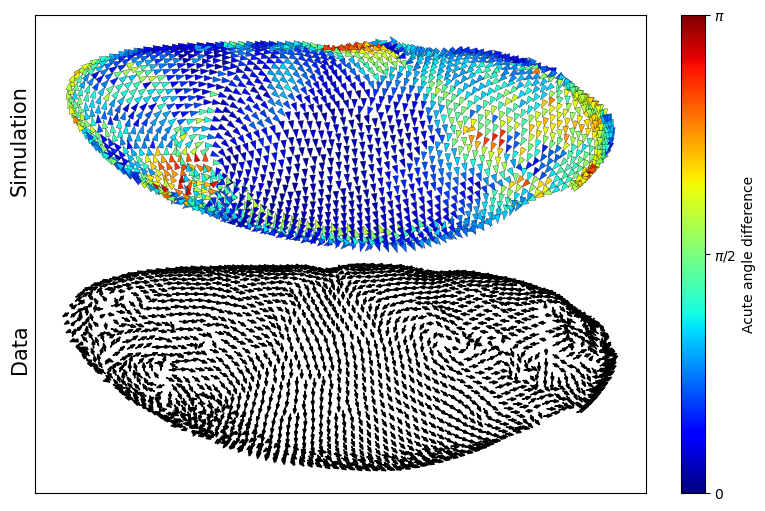
\includegraphics[width=0.9\linewidth]{chapters/Results/figures/movement_vectors_example.png}
    }
    \caption{Snapshot of motion vectors for each cell in simulation and corresponding $\boldsymbol{\mu}_i$. In the simulation each cell is colored according to the angular agreement $\alpha_i$.}
    \label{fig:motionAgreementExample}
\end{figure}


It can be seen that at this specific time point, the agreement ranges from surprisingly good to predictably bad. Visualizing the $\alpha$ metric in this way helps highlight the spatial distribution of the discrepancies. Overall, while large regions display near-perfect alignment, others suggest opportunities for refining the model, particularly it seems like the discrepancies are found in more dynamic regions.\\

\subsubsection{Movement across time}

Now, for ease of parsing, do the following transformation, introducing the metric $\xi_i(t)$:

\begin{equation}
    \xi_i(t=\tau) = 1-\alpha_i(t=\tau)/\pi
\end{equation}

This allows us to score the particles on a scale of 0 to 1, where 0 is no overlap and 1 being perfect alignment with data.\\

Averaging this score over the whole embryo for every time point we get the following relation:

\begin{equation}
     \delta(t) = \frac{1}{N_{cells}} \sum_{i=1}^{N_{cells}}\xi_i(t)
\end{equation}
This number quantifies the average agreement for the embryo at a specific time point. Plotting this we get an estimate of the agreement to the general kinematics of the embryo. In Figure \ref{fig:motionAgreement}, the $\Lambda$-measure can be seen for every time point in the data:

\begin{figure}[H]
    \centering
    \makebox[\textwidth][c]{
    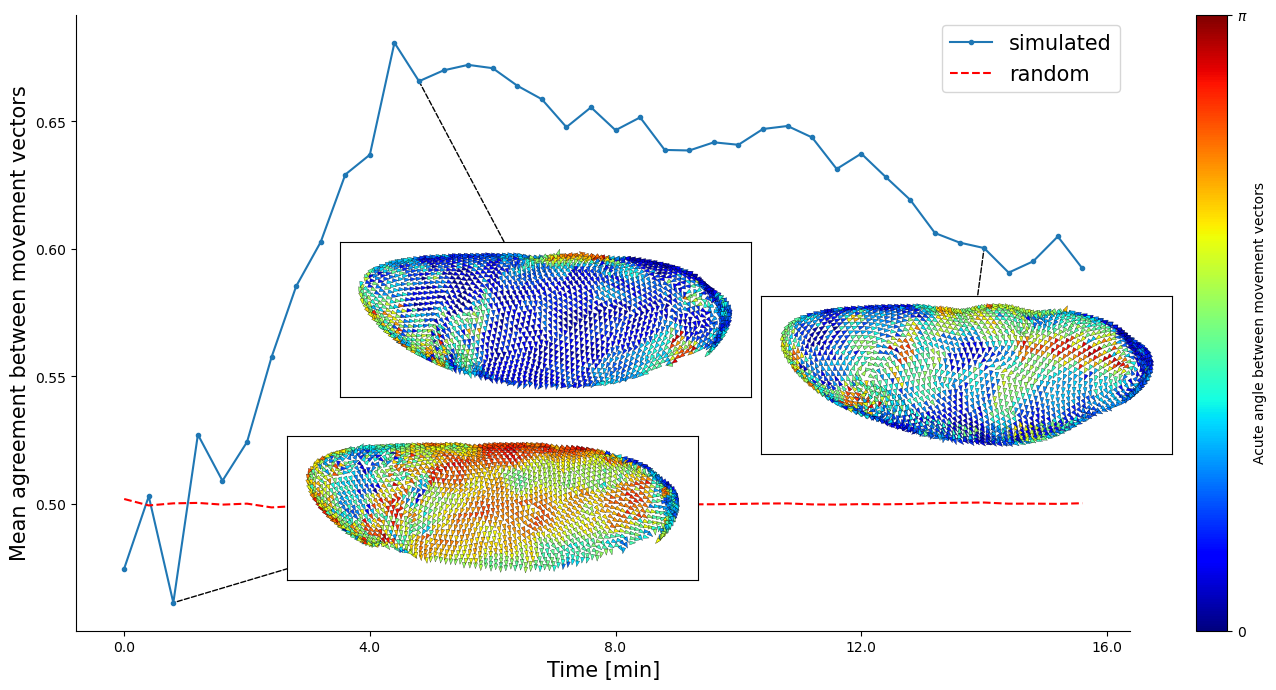
\includegraphics[width=1.3\linewidth]{chapters/Results/figures/movement_vectors_normal.png}
    }
    \caption{The average motion-vector agreement across the full embryo $\delta(t)$ as a function of time. On the inset axes three snapshots of the spatial distribution of error along with the in-simulation motion can be seen.\\
    The red \textit{random}-line corresponds to a simulated embryo where every direction of motion is uniformly randomly chosen.}
    \label{fig:motionAgreement}
\end{figure}


In general, we see a consistent, well-above random overlap between data and simulation. 

From the previous sections, we had some intuition that our simulation visually followed the general flow of the morphogenesis. Figure \ref{fig:motionAgreement} gives us some quantitative confidence that the motion of the individual cells also align with the data. 
Some notes on what we can derive from the above plot:\\

It is very clear that in the first couple of minutes our simulation and reality does not completely agree. This will be a recurring theme. We believe this could be caused by a difference in cell-firmness between real life and our simulation. Specifically, biological cells exhibit a degree of elasticity and plasticity that is not fully represented in our model. When the ventral furrow invaginates (\vf{A1}), the pulling takes some time to stretch each cell, with its center consequently lacking behind. In our model, the tissue moves down immediately and rather uniformly. Taking cell shapes more or less explicitly into account might allow for more gradual stretching, allowing the cells to adjust to tensile forces.\\

Convergent extension is by its very nature based on the global motion being being different from the motion of the individual: For en extension to occur in the horizontal axis, cells will be actively moving along the vertical axis (see Figure \ref{fig:ConvergentExtensionDiagram}). Having a per-cell agreement is almost contradictory to this type of cell motility. This means that for the cell to agree, its surroundings are completely vital. This also doubles as an important argument for doing full-embryo models: When the context [is important] simulating the reciprocity between cell- and embryo-scale motion.\reph\\



\subsubsection{Movement across space}

To find the parts on the embryo that is performing the worst, we look at the integrated error over the full run, summing over every time step.

\begin{equation}
     \label{eq:Delta-measure}
     \Delta_i = \frac{1}{N_{timesteps}}\sum_{\tau = 1}^{N_{timesteps}}\xi_i(t=\tau)
\end{equation}

This results in an "average lifetime error" $\Delta_i$. Mapping this back onto the initial position for cell $i$ we can see how the error is spatially distributed:
\begin{figure}[H]
    \centering
    \makebox[\textwidth][c]{
    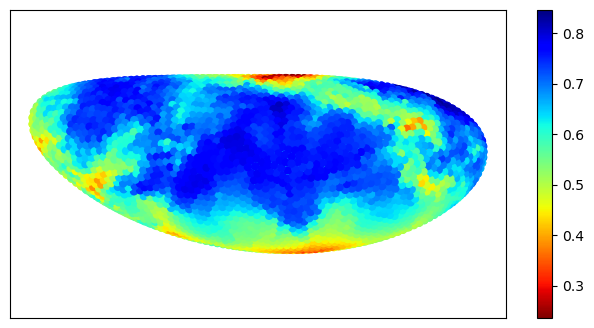
\includegraphics[width=0.9\linewidth]{chapters/Results/figures/movement_mapped_normal.png}}
    \caption{The motion-vector agreement across the full run $\Delta_i$ for each cell $i$ mapped back onto its original positions. Some domains, especially the on the back and belly sides of the embryo, are performing much worse than the rest. }
    \label{fig:}
\end{figure}


A low $\Delta$ indicates a strong match between simulated motions and the mean motion observed by a cell that starts at the corresponding position on the embryo surface. 

Going domain by domain:\\

The in silico motion of the \gb{germ-band} seem in great agreement with data, especially given how far the individual cell travels. We had previously found a qualitative match in overall trajectory and displacement, but this quantifiably highlights the model's ability to capture the large-scale motion of the germ-band extension (\gb{A2}).\\

The \vf{ventral furrow} and its invagination (\vf{A1}) is a main contributor of error. Because of the way the imaging was done, all invaginations (the ventral furrow for example) will automatically have low agreement. The original data only supported motion-tracking on the exterior surface of the embryo.  This limitation naturally reduces the precision of our comparisons in regions where inward movements are critical, which is one of the primary types of motion. \\

On top (the dorsal side), the sheet buckles and folds in vivo. This was not part of our simulation and it can also be seen that our measure of agreement is greatly penalized.\\

For the \pmg{posterior} part of the embryo, the agreement is suprisingly good. This is either because the cells that start at this positions makes the general motion albeit not far enough (remember displacement magnitude does not matter), or the no-inward-motion-tracking is somehow doing us a favor.\reph\\


Finally, the head part of the embryo (left of the \cephalic{cephalic furrow}), especially on the lower side, a lot of error accumulates. The head area was from the start deemed outside the scope of the current project, so quite a lot of disagreement is anticipated.\\


\subsubsection{Movement across domains}
Having such a large discrepancy at specific parts of the egg gives us the idea of discarding parts of the egg from the calculation.\\


We calculate the mean agreement-score $\delta(t)$ just like in Figure \ref{fig:motionAgreement}, but this time excluding cells, in the \cephalic{cephalic} area, in the \vf{ventral furrow}, or both:



\begin{figure}[H]
    \centering
    \makebox[\textwidth][c]{
    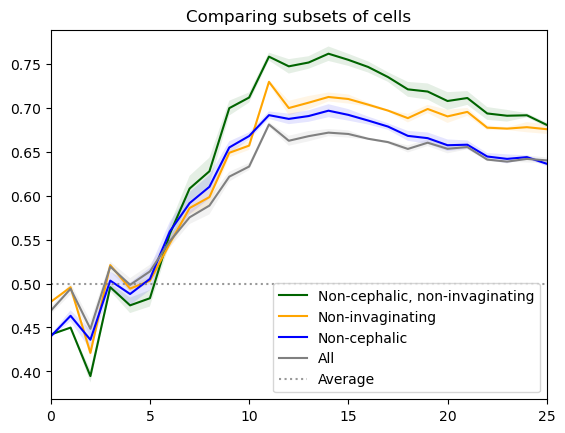
\includegraphics[width=1\linewidth]{chapters/Results/figures/movement_vectors_normal_subsets.png}}
    \caption{The motion-vector agreement across the full embryo $\delta$ but with certain domains excluded from the calculation. For confidence in the stability of the solution, all lines and shaded areas are averages and and standard deviations of three runs using identical parameters but different seeds.\\It is clear that excluding some domains improves the general agreement.}
    \label{fig:vector-subsets}
\end{figure}

As can be seen in Figure \ref{fig:vector-subsets}, limiting the agreement analysis to only look at specific subsets of the embryo improves the performance significantly:\\

Once anything in the head area is discard from the average (\cephalic{Non-cephalic}), we see a noticeable bump in quality. This is true for the most of the duration, but the effect is actually reversed in the far ends of the simulation. We believe this occurs because of the relatively well-behaved cephalic region --  excluding it helps boost the overall average when other regions perform well. However, when the rest of the simulation decline, removing the head slightly heightens the average quality. \\

Removing cells in the Ventral areas that were apically constricting (\vf{Non-invaginating}) we see an even more pronounced increase. This time, the increase is, predictably, more stable, as these areas are responsible for consistently worse performance. \\

Combining both masks (removing both the head-region and the  invaginating parts) gives an even better result. [something something averages] \\


To summarize: Focusing on the parts of the embryo with a good possibility of overlap with data, we get a much higher average cell-motility agreement (almost 0.8) during the dynamic phases of the simulation. The improvements are substantial and we feel it helps portray how our model can excel.

\subsection{Strain}
As the tissue warps and skews, the cells are both subject to- and drivers of- stress and strain on the cell walls. These mechanics are some of the most widely studied parts of the in morphogenesis.\\

While our simulation neither includes cell walls nor explicit strain calculations, a method has been developed that only requires positions of cell-centers -- and that we have! The Green-Lagrangre algorithm (implemented as described in \citeAY{butler2009cell}), can be applied to find local deformations in tissue. In Figure \ref{fig:strain} the results of an implementation can be seen and compared to a graph on data.
\begin{figure}[H]
    \centering
    \begin{subfigure}{0.45\linewidth}
        \centering
        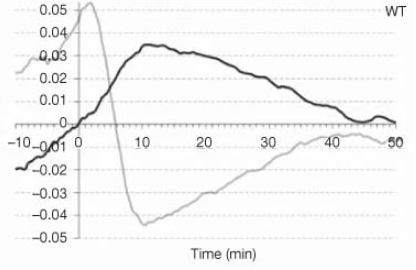
\includegraphics[width = \linewidth]{chapters/Results/figures/strain_rate_extrinsic2.png}
    \end{subfigure}
        \begin{subfigure}{0.45\linewidth}
        \centering
        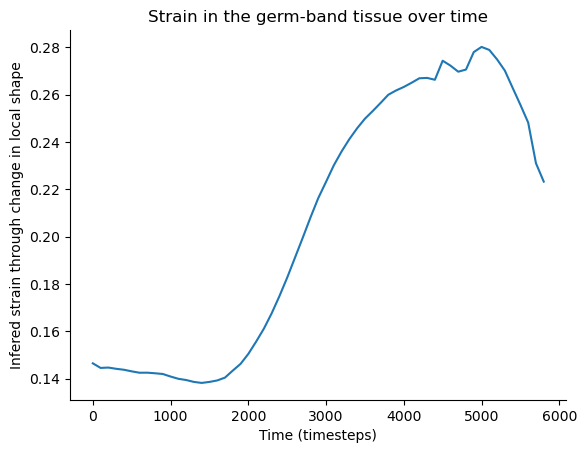
\includegraphics[width = \linewidth]{chapters/Results/figures/strain_smoothedpng.png}
    \end{subfigure}
    \caption{A comparison of estimated strain-rates as a function of time between in-vivo data and our simulation. In both cases we see a quick rise followed by a fall-off at the time of invagination of the posterior (\pmg{A3}) at around 12 minutes. \\\textbf{Left}: A plot of the inferred strain rate (black line) in the germ-band (Source: \citeAY{butler2009cell}). \\\textbf{Right}: The inferred strain rate in simulation using the the Green-Lagrangre algorithm.\\
   }
    \label{fig:strain}
\end{figure}

In the first 12-15-minutes we see a rising strain, ending at the point of internalization of the germ cells (\pmg{A3}). In our simulation, the strain has a delayed onset, once again showing how the first 2 minutes have a central difference from ground truth. To remind, we previously postulated this was due to overly rigid tissue in simulation, which would also explain the too low local strain. \\

This section allows for a great comparison, as it highlights a fundamental discrepancy in tissue mechanics between our model and actual biological behavior. We have previously found a great visual agreement between simulation and data, but we now YYY, that we have while not being able to run from the fact that some of the fundamental physics YY.\reph 

Despite the overall success of the simulation, this divergence in strain accumulation suggests that the mechanical/viscoelastic properties of the tissue are not fully captured and might require further refinement. 



\newpage
\section{In Silico Mutants}
Having a complete simulated pipeline from (simplified) morphogen to (approximate) morphogenesis, opens the door for some intriguing explorations into our model and its relation to nature. \\


A large branch of developmental biology consists of discovering or creating mutated embryos, examining the resulting organisms, thereby learning something about the translation from DNA, through cellular mechanics, to finished animal.\cite{gilmour2017morphogen}\reph
Our model also allows for the creation of genetically-variant embryos by changing the response to one or more of the simulated morphogens. In theory, we can make \textit{predictions} by analyzing how variations in morphogen distribution or cell interactions affect morphogenesis in our simulation. We might be able to gain insights that could inform or direct experimental studies.\\

We have seen how a visually and analytically [compelling] 3-dimensional recreation is possible. Having a framework for both simulation and analysis, we will now inspect the interplay between different actions and interactions between different places.\reph?\\



\subsection{The mutants}
To introduce this section we will need to shortly explain the most interesting "mutants" that incidentally hinder \vf{A1}, \gb{A2} and \pmg{A3} respectively. Their mechanics and morphologies will be briefly explained, and the implications for our model briefly explored. \\
Videos of the individual runs can be found in Section \ref{App:videos} in the Appendix.

\subsubsection{(\vf{A1}) No Ventral Furrow }
When knocking out the \textit{Twist} and \textit{Snail} genes, which are primary organizers of apical constriction, the ventral furrow fails to form (stage \vf{A1} on Figure \ref{fig:big-timeline}).\cite{leptin1991twist} \\

Due to the interconnectedness of the different parts of the embryogenesis, the lack of invagination on the belly (\vf{A1}) also disrupts posterior midgut invagination (\pmg{A3}), altering the expected shape. Surprisingly, the resulting organism remains viable.\cite{conte2012biomechanical} This comes down to the fact, that nature is resilient and the embryo still manage to invaginate the pole cells at the posterior, although the timing and morphogenetic movements are significantly disrupted. In \citeAY{zusman1988short}, it is shown that, as a reaction to the missing invagination, an activation of the gene \textit{sog} delays the process by approximately six minutes in an attempt to compensate for the disrupted gastrulation, further highlighting both the temporal sensitivity and interconnectedness of these developmental events.\\

We were unable to find any videos of this mutant, but our simulation can be seen in Figure \ref{fig:VFmutant} below:

\begin{figure}[H]
    \centering

    \makebox[width = 1.\linewidth][c]{
    \centering
    \hspace{-2cm}
    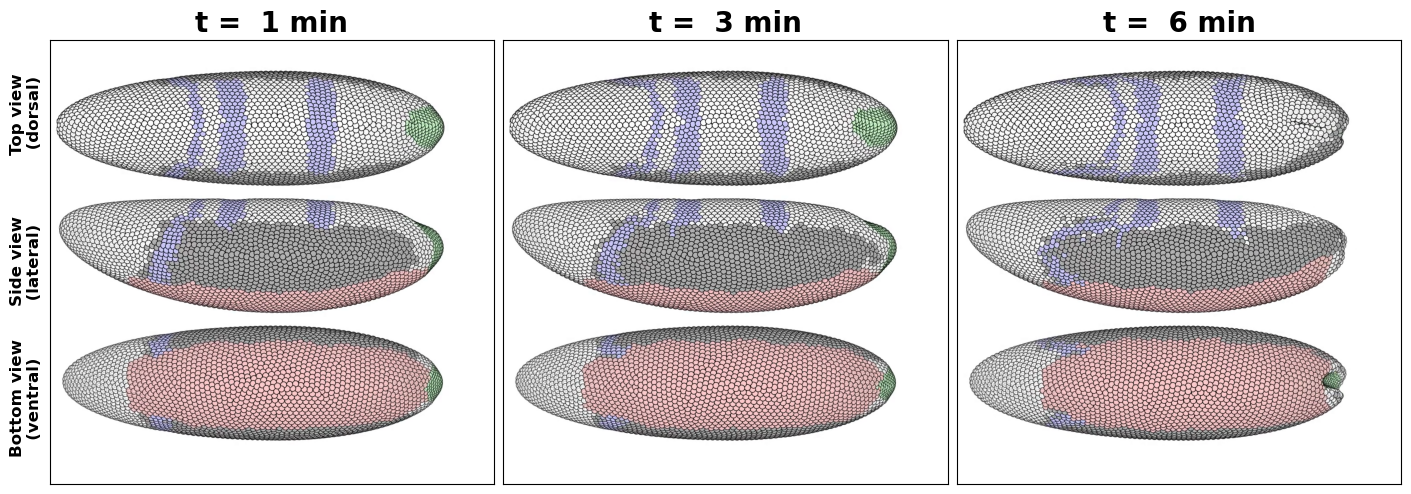
\includegraphics[width=1.3\linewidth]{chapters/Results/figures/noVF.png}}
    \caption{Three snapshots of the model simulating gastrulation, but the without the virtual gene activating ventral furrow formation (\vf{A1}). The colors correspond to different cell types. It can be seen that the germ-band still extends horizontally (\gb{A2}), but the posterior midgut does not invaginate correctly (\pmg{A3}) and is not moved upwards, away from the belly.}
    \label{fig:VFmutant}
\end{figure}


In simulation the lack of \vf{ventral furrow} on the belly, results in the germ-band not moving downwards. As these is no compensating genetic factors in our simulation, the pressure exerted by the extending germ-band \gb{A2} is unable to move the posterior much "upwards". This results in an invagination at the tip after about 6 minutes, after which the germ-band is moved up slightly. This can be seen in Figure \ref{fig:VFmutant}.\\



% \todo{cite \citeAY{lye2024polarised}}
% \textit{As tissues grow and change shape during animal development, they physically pull and push on each other, and these mechanical interactions can be important for morphogenesis. During Drosophila gastrulation, mesoderm invagination temporally overlaps with the convergence and extension of the ectodermal germband; the latter is caused primarily by Myosin II–driven polarised cell intercalation. Here, we investigate the impact of mesoderm invagination on ectoderm extension, examining possible mechanical and mechanotransductive effects on Myosin II recruitment and polarised cell intercalation. We find that the germband ectoderm is deformed by the mesoderm pulling in the orthogonal direction to germband extension (GBE), showing mechanical coupling between these tissues. However, we do not find a significant change in Myosin II planar polarisation in response to mesoderm invagination, nor in the rate of junction shrinkage leading to neighbour exchange events. We conclude that the main cellular mechanism of axis extension, polarised cell intercalation, is robust to the mesoderm invagination pull. We find, however, that mesoderm invagination slows down the rate of anterior-posterior cell elongation that contributes to axis extension, counteracting the tension from the endoderm invagination, which pulls along the direction of GBE.}
% \url{https://genesdev.cshlp.org/content/5/9/1568.full.pdf}
% We are seeing the right thing
% Comparing We are seeing the right thing.



% \subsection{Auxiliary(cephalic furrows}

% In the absence of controlled folding of the dorsal tissue, the pressure from the extending Germ Band, can lead to other folds(?) \url{https://brunovellutini.com/posts/cephalic-furrow-thread/}

% This is key to both understanding why the invaginated posterior end does not travel further anteriorly.

% Also the large scale morphology change some runs had.

\subsubsection{(\gb{A2}) No Germ-band }
\label{sec:mutantNoGB}
When removing the patterning that is believed to be responsible for convergent extension in the germ-band, something surprising happens. It has been show that Drosophila morphogenesis is driven by more than convergent extension, and that \gb{germ-band}-lacking-mutants are still viable: In \citeAY{butler2009cell} they show that active cell elongation overtakes the responsibility for moving the tissue and the gastrulation proceeds almost uninterrupted.\\

In our simulation, we have no cell shape change to help alleviate the lack of motion, but as the ventral furrow without interruption invaginates (\vf{A1}), some movement is still seen. 
Again, unable to find any videos of this mutant, Figure \ref{fig:VFmutant} simply shows our model.

\begin{figure}[H]
    \centering

    \makebox[width = 1.\linewidth]{
    \centering
    \hspace{-2cm}
    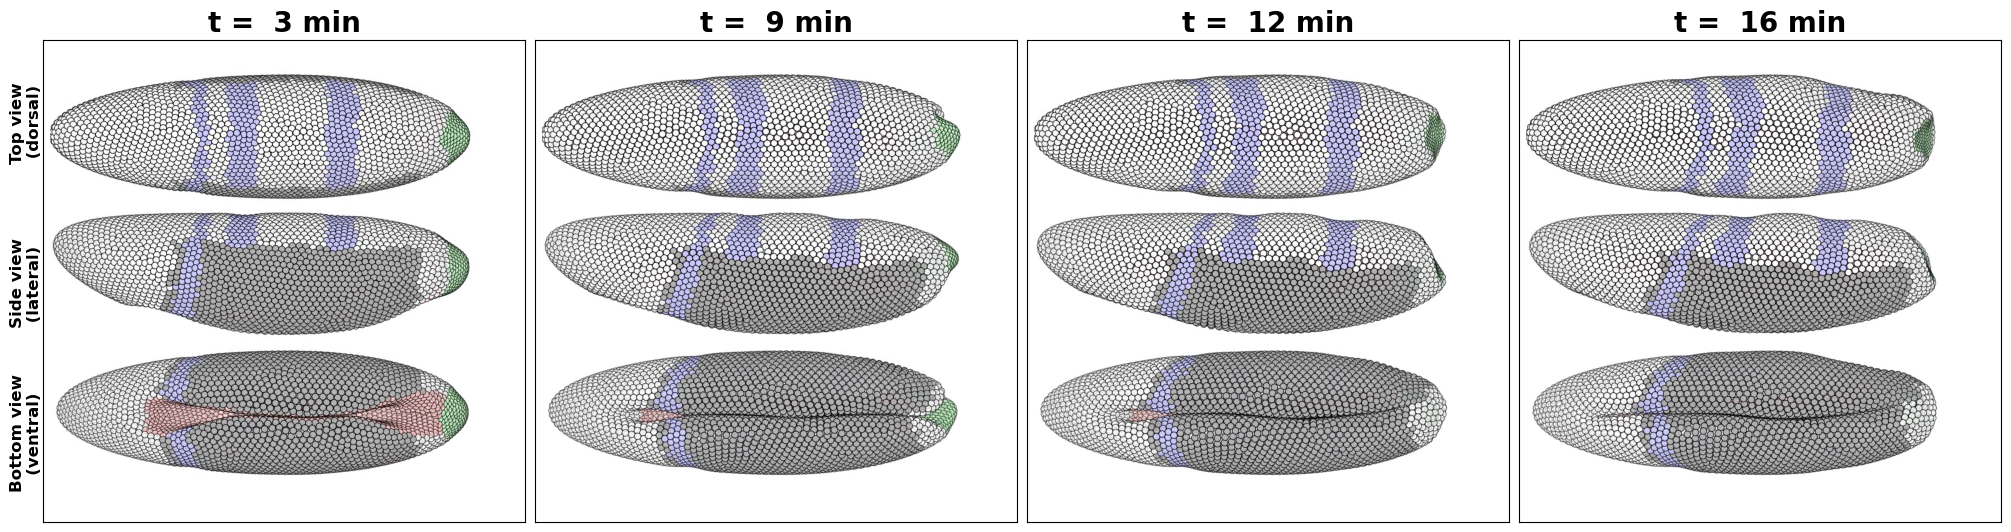
\includegraphics[width=1.3\linewidth]{chapters/Results/figures/noGB.png}
    }
    \caption{Three snapshots of the model simulating gastrulation, but the without the virtual gene activating germ-band exension (\gb{A2}). The ventral furrow forms as normal (\vf{A1}), but the posterior midgut is not internalized (\pmg{A3}) and neither it nor the germ-band are moved upwards.}
    \label{fig:germ-band-mutant}
\end{figure}


% Left right anisotopri

Especially interesting is the following: As the posterior contracts in an attempt to internalize, it is not moved away from the narrow boundary condition on the tip, making the invagination impossible. This is a clear testament to the importance of not only having  connections to the surrounding tissue, but also having an full-3D model of the boundary condition, as the resulting morphological movements are highly spacial in nature and therefore non-trivial to capture in a less specific(?) simulation. As we have no references for a "no germ-band and no ventral furrow"-double mutant, in a moment of hubris we might even propose the above behavior as a qualitative prediction for a possible biological experiment.\\  
A final thing to note: As the posterior is not moved upwards, we observe slight twisting of the tissue during the process (this is a clever way to segue to the next section). 


\subsubsection{(\pmg{A3}) No Posterior Midgut Invagination(PMG)}
The PMG is the name for the invagination that happens at the posterior to internalize the pole cells (\pmg{A3} on Figure \ref{fig:big-timeline}).

In [cite Stas], they show that a chemical signal from the protein \textit{Hkb} initiates constriction on the posterior tip. In \textit{Hkb}-deficient mutants the lack of posterior invagination has a clear effect: The built up pressure from the extending germ-band causes the whole to twist. This has given the \textit{Hkb}-mutant the nickname "Corkscrew".\\

This time we are lucky as there is a full video of the resulting mutant available. In Figure \ref{fig:corkscrew-comparison}, the video of a 'corkscrew mutant' can be compared to our simulation after removing the ability for the posterior to invaginate.

 
\begin{figure}[H]
    \centering
    \makebox[\textwidth][c]{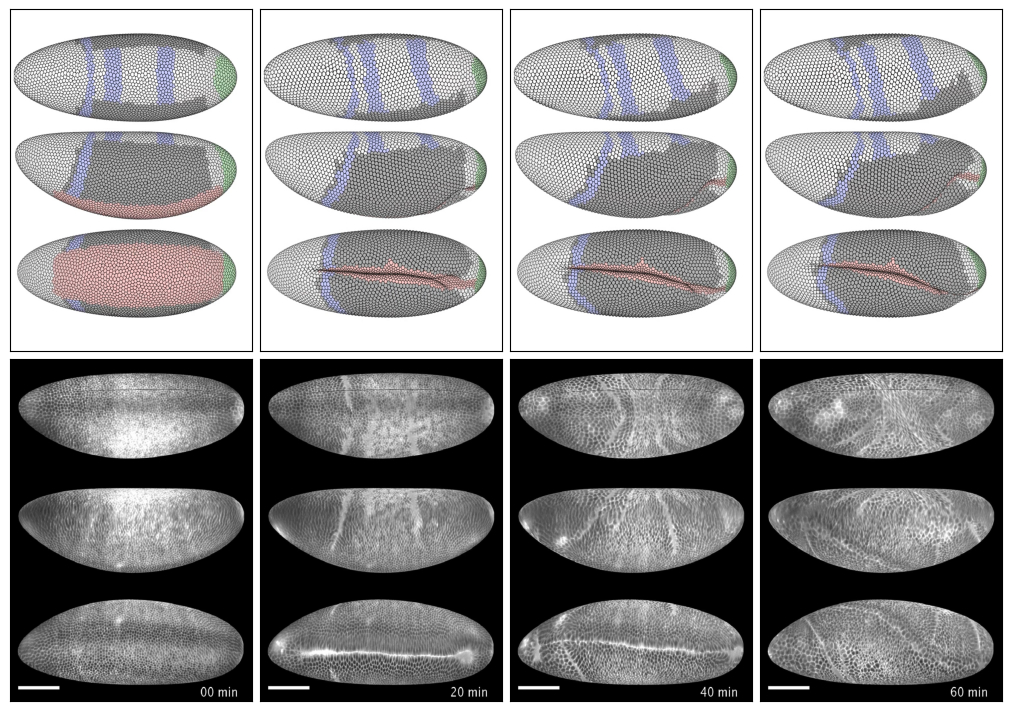
\includegraphics[width=1.2\linewidth]{chapters/Results/figures/corkscrew_comparison.png}}
    \caption{A purely visual comparison of the \textit{Corkscrew} phenotype.\\
    \textbf{Top:} Simulation colored by cirtual cell type. \\
    \textbf{Bottom:} Light sheet imaging of cell walls (Source: \citeAY{smits2023maintaining})\\ In both cases  a "twisting" motion can be seen. This is most noticeable when paying attention to the line formed by the ventral furrow.}
    \label{fig:corkscrew-comparison}
\end{figure}
% Twist and shout

 The in vivo and in silico mutant visually agree on the motion, albeit on different time scales. Comparing the lines formed by the ventral furrow on the belly of the embryo, we can see twisting phenomenon present in vivo and is also present in our in silico models. As we did not design the model for this express purpose, it suggests that some fundamental tissue dynamics might be captured by the simulation. \\


In general, comparing the reaction of these in silico mutants to real life phenotypes gives us a hint that our model has a somewhat correct [smth] of principles governing the cellular behavior, while also showing some fundamental differences. \reph

% This suggests that the broader processes driving morphogenesis may rely more on spatial and interaction rules than on precise timing."

% We know that \textit{Runt} and \textit{Even skipped} are upstream . The litterature is conflicted, but the general theory is, that the patterning allows for a coherent orientation of the planar cell polarity. 

% PCP-orientation was set at the intial step of the simulation as pointing in the distinct direction defined by the interspersed \textit{Runt} and \textit{Even skipped} patterning.
% The results are interesting, albeit very uneventful, as
% In the litterature  \cite{butler2009cell} more the morphogenesis is driven by more than Convergent Extension, and unstriped mutants are still viable, unlike our case where nothing happens.

% Seems to be a clear indicator for active cell shape change being a vital part of... 

% TODO: Discuss level of abstraction in the model 

\subsection{Combining and Comparing to Benchmark}


Given that we have the world’s first full embryo model, we can conduct some interesting in-silico experiments. A particularly fascinating aspect of morphogenesis across all species is the interplay between the various spatially separated regions of the embryo. To our knowledge, the ability so see the reaction in passive regions by their dynamic neighbors has not been a focus of any previous in silico experiments.  In this section, we will analyze how these regions interact and influence each other and the final outcome.

We will be doing this analysis in two tways: Firstly by comparing the different virtual 'phenotypes' to our in silico baseline. Secondly by comparing to the in vivo motion data.  

\subsubsection{Pole Cell Migration}
We will start out by introducing the metric \textit{Pole Cell Migration} as a virtual quantification for the success of the gastrulation. The Pole Cell Migration (PCM) is defined as the angle change of the posterior tip in the lateral plane. That is, in degrees, how far around the embryo the posterior has moved. In Figure \ref{fig:PCM_diagram} this is sketched out.  \\


\begin{figure}[H]
    \centering
    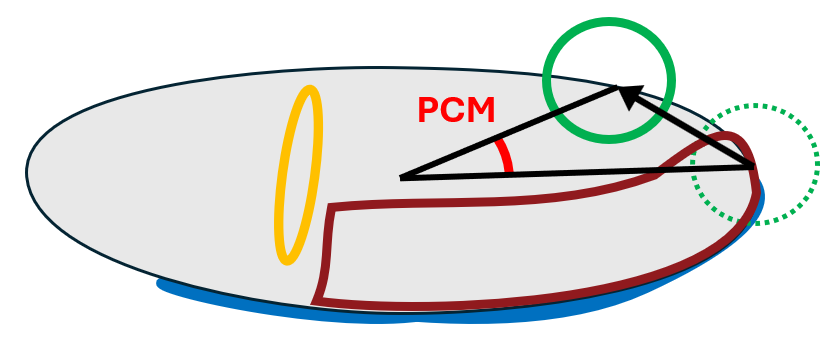
\includegraphics[width=0.75\linewidth]{chapters//Results//figures/PCM_diagram.png}
    \caption{A diagram of the calculation of the PCM-metric.
    The primary domains are drawn in in.\\
    PCM is calculated as the angle between center of embryo and inital and final position of the posterior tip respectively.}
    \label{fig:PCM_diagram}
\end{figure}

Using the above metric, we can condense one of the main motions of the gastrulation (the translation of the posterior tip to the back-side) down to a single number. In Figure \ref{fig:PCM-mutants} a comparison of multiple runs of the known mutants described earlier can be seen and compared to the wild-type.

\begin{figure}[H]
    \centering
    \makebox[\linewidth]{
    \begin{subfigure}[t]{0.9\linewidth}
            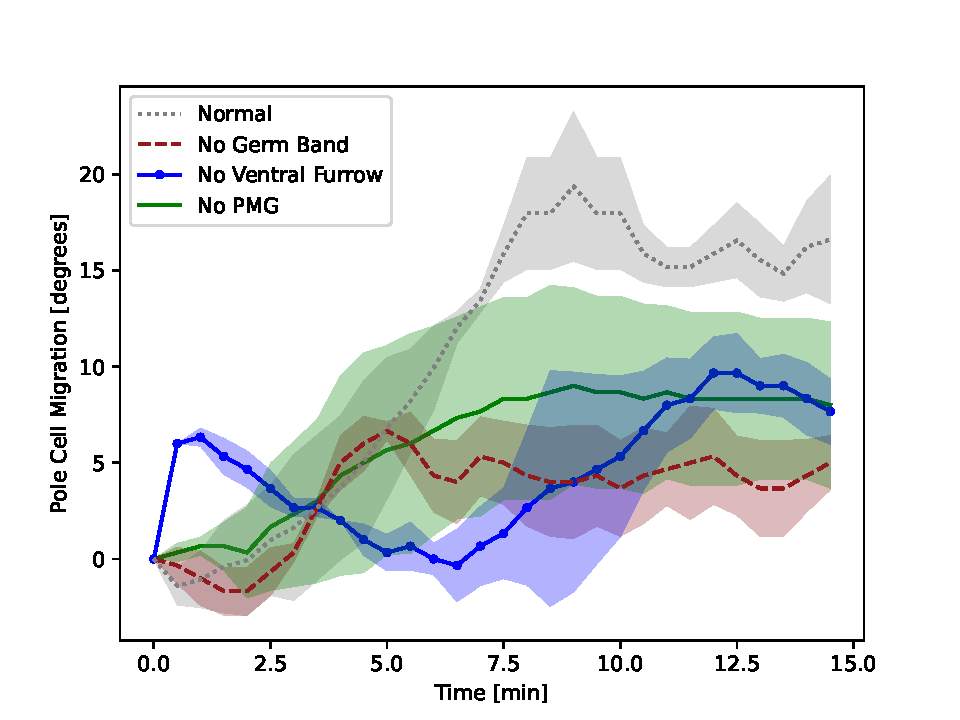
\includegraphics[width=1.\linewidth]{chapters/Results/figures/compare_PCM.pdf}
    \end{subfigure}
    \hspace{-1.2cm}
    \begin{subfigure}[t]{0.45\linewidth}
    
            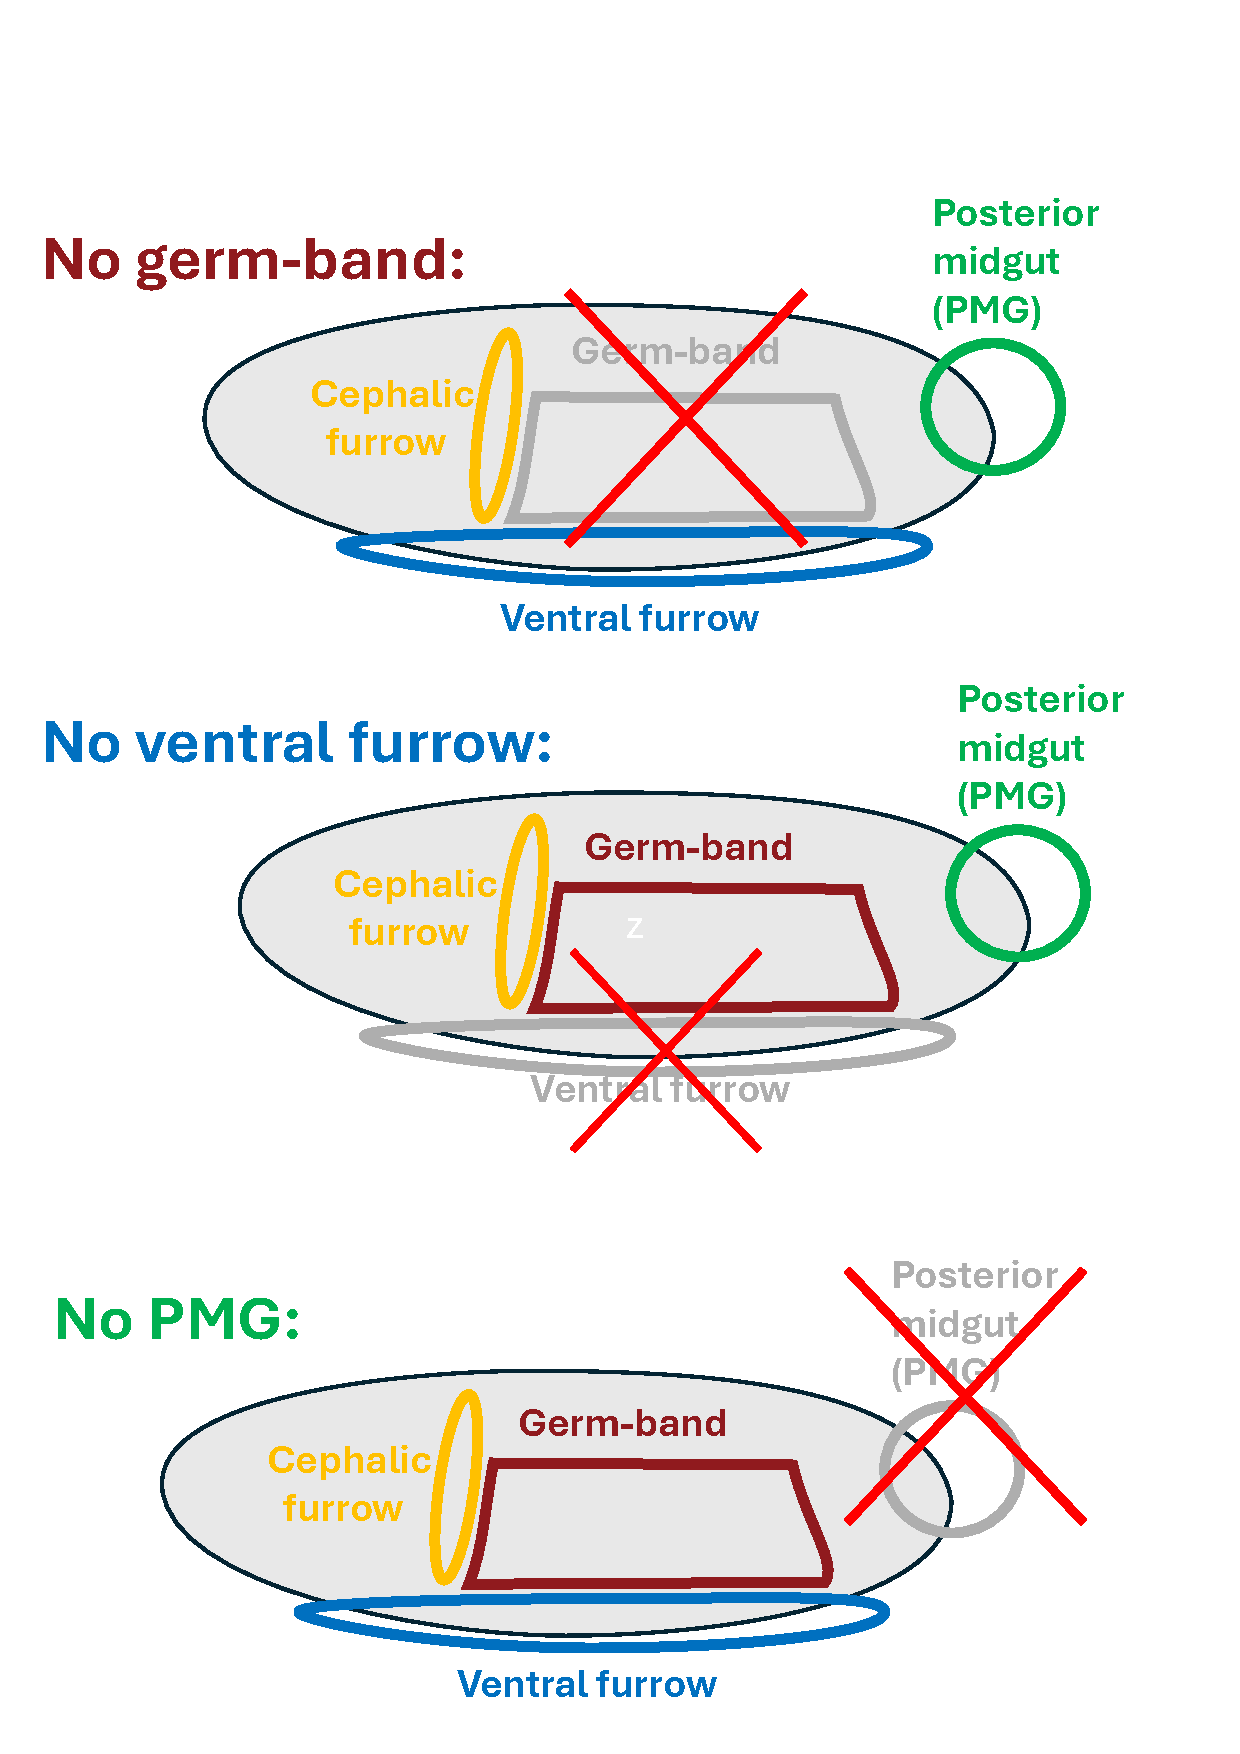
\includegraphics[width=1.\linewidth]{chapters/Results/figures/mutant_diagrams.pdf}
    \end{subfigure}
    }
    \caption{\todo{Explain,}}
    
    \label{fig:PCM-mutants}
\end{figure}


The mutants has been individually explained earlier, but a lot of the dynamics of the system can be gathered from the motion of the posterior tip. At risk of repeating ourselves, we can see that:\\
\begin{description}
    \item[Normal (\textcolor{darkgray}{grey}):] This is the normal run. A ramping movement until reaching the point of posterior invagination just below 20 degrees. 
    \item[No germ-band (\gb{red}):] At first the tip moves downwards towards the invaginating ventral furrow. When the belly convergently extends, there is a tendency to move the tip dorsally, but there is not enough force for the posterior tip to progress more than 5 degrees. 
    \item[No ventral furrow (\vf{blue}):] Firstly, when no tissue is pulled into the bottom side, the germ-band pushes the posterior tip 'from the sides' instead of from the bottom. This results in a slight upwards motion in the PCM followed by an \todo{finish}. In real life, after a delay, the system is overdetermined and other actions overtakes to eventually shift the posterior upwards, allowing the process to proceed. Interestingly, even with this altered timing and mechanical dynamics, the posterior region still manages to achieve its upward shift, and the embryo remains viable. 
    \item[No PMG (\pmg{green}):]  Here we see a possible breakdown of this metric. None of the corkscrew-twisting is captured and the lowering of PCM does not capture just how unviable an embryo with this mutation is.  
\end{description}

This section was mainly included to show the potential of having a quantifiable metric Ala PCM. Because of the generality of the pipeline we have set up, in the future, a more complex simulation including more active events, folds etc. can have easily have their 'mutants' added to this graph simply by defining which gene-responses to disregard. Having a numerical criterion would also allow for intersections (both removing \vf{A1} and \gb{A2}, for example) to be measured against a benchmark.
% \begin{wrapfigure}{l}{0.\textwidth}
%     \centering
%     \hspace{-3cm}
%     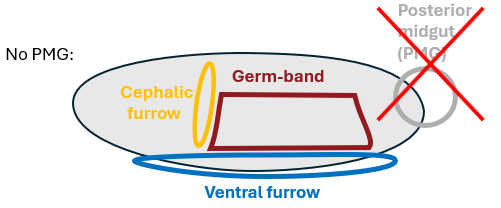
\includegraphics[width=0.5\linewidth]{chapters//Results/no_pmg_mutant_schematic.png}
% \end{wrapfigure}


\subsection{Combining and comparing to Data}
While comparing models internally is interesting and can say a lot about the dynamics, we wanted a short detour, recreating Figure \ref{fig:motionAgreement}, seeing how each mutation changes the motion-vectors. The results can be seen in Figure \ref{fig:compare-motionAgreement-time} below:

\begin{figure}[H]
    \centering
    \makebox[\textwidth][c]{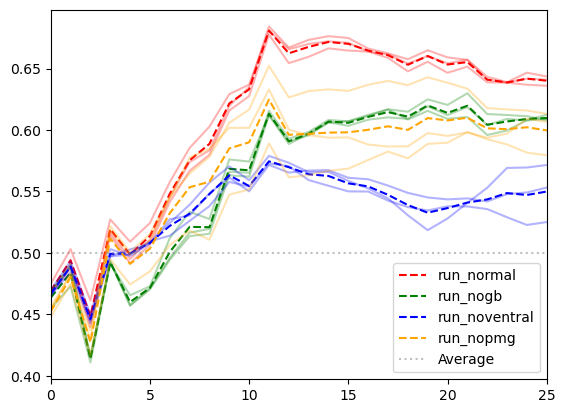
\includegraphics[width=1.3\linewidth]{chapters/Results/figures/PLACEHOLDER_compare_movement_vectors.png}}
    \caption{ Y-axis defined like Figure \ref{fig:motionAgreement}. \todo{This is an important plot. Remake in higher quality with  better legend and axis labels}}
    \label{fig:compare-motionAgreement-time}
\end{figure}
It is comforting to see that the motion agreements are all above-random but below the normal benchmark.\\

The "No Germ-band"-mutant is surprisingly good. We think this is due to the fact that only the angles between the motions matter: If the cell-sheet moves along the right direction, it does not matter whether the sheet moves far enough or fast enough.\\

Removing the ventral furrow is by far the most disruptive perturbation to the embryo when looking at these displacement vectors. This is explained by the fact that the downwards movement (towards the ventral furrow) is characteristic. The fact that the mutant lacking a ventral furrow invagination is performing better than the germ-band-less mutant corroborates the previously proposed idea that our germ band is pulled downwards too far too quickly.\todo{check if this is actually mentioned before}\\

To become more certain of any the above explanations, we can look at the temporal [], finding the combination of time and space where the different part of the embryo are important. In Figure \ref{fig:compare-motionAgreement-space} below, we have quantified the motion-vector agreement for the best run of our model at thee different time points and mapped it back onto the original embryo. This is then also done for the different, above mentioned, mutants, and the difference is visualized. 
\begin{figure}[H]
    \centering
    \makebox[\textwidth][c]{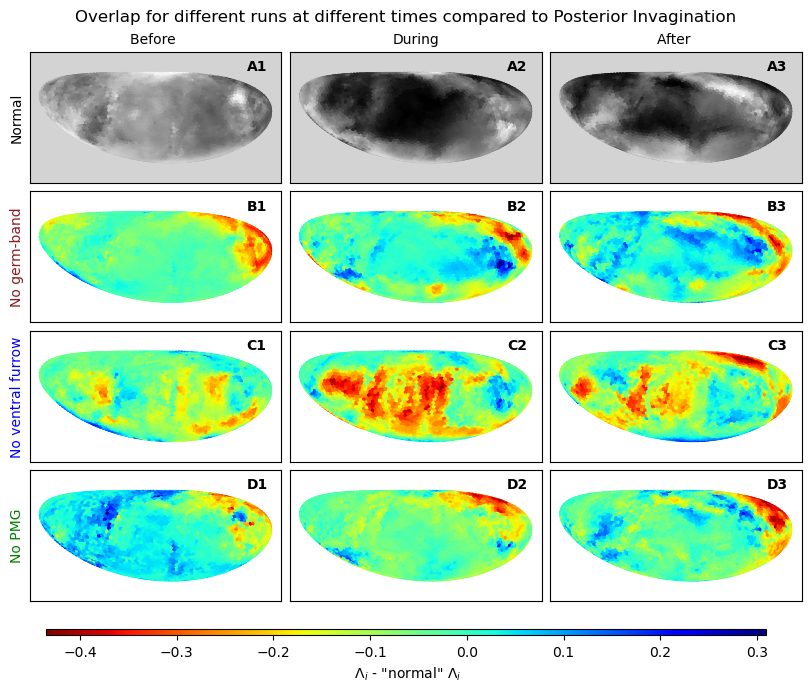
\includegraphics[width=1.3\linewidth]{chapters/Results/figures/Compare_all_movements_annotated.png}}
    \caption{The diference in the $\Delta$ measure (as defined in Equation \ref{eq:Delta-measure}) for three virtual mutants and the unperturbed gastrulation. Top row has different color scale where white is high disagreement. 
    It can be seen that disrupting a morphogenetic event has cascading errors that greatly affect the accuracy of other, separate events.}
    \label{fig:compare-motionAgreement-space}
\end{figure}
\newpage

We can use Figure \ref{fig:compare-motionAgreement-space} to do the combined: When, where, and how much are each mutation disruptive for the normal flow of gastrulation. 

We inspect it row by row:

\begin{description}
    \item[Normal:] The \textit{normal} run has already been discussed. We are here using it as a be a benchmark/reference. 
    \item[\gb{No germ-band}:] The absence of an active germ-band proved to be less problematic than initially expected.The current analysis reveals that a large part of the germ-band's agreement with reality was due to its downward motion. It is very clear though, that the posterior tip --  which had a great agreement in the \textit{normal} run -- is acting much worse when comparing to data. In previous sections, it was clear that this mutation disrupted the posterior midgut (PMG), leading to observable changes. Curiously, the small diagonal band between germ-band and posterior that originally had now agreement (as can be seen in \textbf{A3}) has improved. This might be some complex interaction between the posterior and the lateral sides of the embryo, but it could also be a sign that our implementation of the active germ-band has some room for improvement.\\
    \item[\vf{No ventral furrow}:] As already seen in Figure \ref{fig:compare-motionAgreement-time}, removing the ventral furrow has by far the most severe impact for the simulation’s ability to reproduce "normal" gastrulation. The ventral furrow is critical in the first large-scale movement and, in our simulation, vital for directing the germ-band. Without it, our model struggles to simulate the correct spatial deformations. It has been experimentally shown that the active convergent extension in the germ-band is in neither dependent on nor affected by the pulling force from the invagination on the lower side of the embryo.\cite{lye2024polarised} 
    \item[\pmg{No PMG}:] Removing \pmg{PMG} leads, unsurprisingly, to significant simulation errors at the posterior end -- a place where our simulation so far has seemed to be quite well aligned with data. Surprising is it, that it seems as if the performance in the head area (left of the \cephalic{cephalic} furrow) is quite significantly improved.
    It seems the lack of relief of pressure towards the back side will improve the front.  
\end{description}

The fact that loosing \vf{A1} gave a much higher error in the germ-band, loosing \gb{A2} a lot higher error in the PMG, and loosing \pmg{A3} improved the front part of the embryo, helps elucidate the fact of complementary and interdependent domain- and event- interactions!



% \section{Interaction Matrix}
% For a more granular approach, we boil the PCM down to a single number quantifying the total dorsal motion. In the matrix in Figure \ref{fig:PCM-matrix} the combined effects of missing any two can be seen (once i make it) together with the data-quantified overlaps:
% % \footnote{emitting about 7kg of CO2 \url{https://mlco2.github.io/impact} }
% \begin{figure}[H]
%     \centering
%     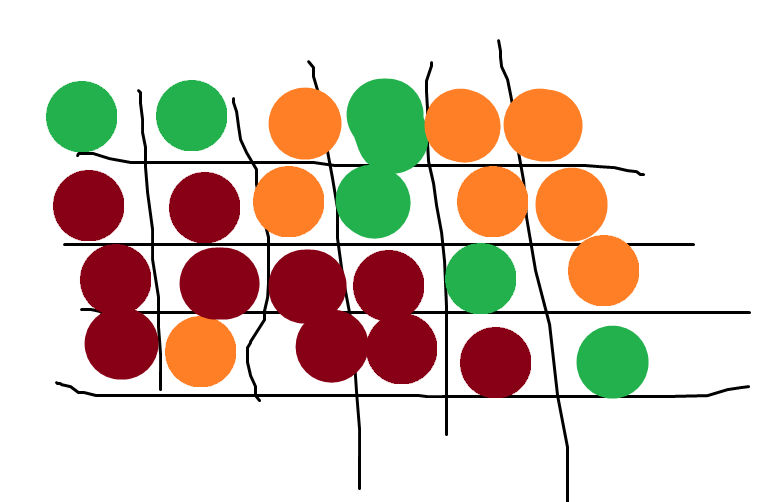
\includegraphics[width=1.\linewidth]{chapters/Results/figures/placeholder_domain_matrix.png}
%     \caption{Not done yet}
%     \label{fig:PCM-matrix}
% \end{figure}

% \todo{Find something interesting to discuss}


% \section{Without gene-defined PCP-initialization}
% \todo{Cut for time or make for appendix}



% \url{https://softmath.seas.harvard.edu/wp-content/uploads/2019/10/2009-07.pdf}
% clear that model is missing cell shape change!
% \section{Additive/subtractive working together matrix}
% \subsubsection{}